
\chapter{Inference for categorical data}
\label{inferenceForCategoricalData}

Chapter~\ref{inferenceForCategoricalData} introduces inference in the setting of categorical data. We use these methods to answer questions like the following:
\begin{itemize}
\setlength{\itemsep}{0mm}
\item What proportion of the American public approves of the job the Supreme Court is doing?
\item The Pew Research Center conducted a poll about support for the 2010 health care law, and they used two forms of the survey question. Each respondent was randomly given one of the two questions. What is the difference in the support for respondents under the two question orderings?
\end{itemize}
We will find that the methods we learned in previous chapters are very useful in these settings. For example, sample proportions are well characterized by a nearly normal distribution when certain conditions are satisfied, making it possible to employ the usual confidence interval and hypothesis testing tools. In other instances, such as those with contingency tables or when sample size conditions are not met, we will use a different distribution, though the core ideas remain the same.


%__________________
\section{Inference for a single proportion}
\label{singleProportion}

\index{data!supreme court|(}

According to a New York Times / CBS News poll in June 2012, only about 44\% of the American public approves of the job the Supreme Court is doing.\footnote{\href{http://www.nytimes.com/2012/06/08/us/politics/44-percent-of-americans-approve-of-supreme-court-in-new-poll.html}{\scriptsize nytimes.com/2012/06/08/us/politics/44-percent-of-americans-approve-of-supreme-court-in-new-poll.html}} This poll included responses of 976 adults.


\subsection{Identifying when the sample proportion is nearly normal}

A sample proportion can be described as a sample mean. If we represent each ``success'' as a 1 and each ``failure'' as a 0, then the sample proportion is the mean of these numerical outcomes:
\begin{eqnarray*}
\hat{p} = \frac{\ 0 + 1 + 1 + \cdots + 0\ }{976} = 0.44
\end{eqnarray*}
The distribution of $\hat{p}$ is nearly normal when the distribution of 0's and 1's is not too strongly skewed for the sample size. The most common guideline for sample size and skew when working with proportions is to ensure that we expect to observe a minimum number of successes and failures, typically at least 10 of each.

\begin{termBox}{\tBoxTitle{Conditions for the sampling distribution of $\hat{p}$ being nearly normal}
The sampling distribution for $\hat{p}$, taken from a sample of size $n$ from a population with a true proportion $p$, is nearly normal when
\begin{enumerate}
\item the sample observations are independent and
\item we expected to see at least 10 successes and 10 failures in our sample, i.e. $np\geq10$ and $n(1-p)\geq10$. This is called the \term{success-failure condition}.
\end{enumerate}
If these conditions are met, then the sampling distribution of $\hat{p}$ is nearly normal with mean $p$ and standard error
\index{standard error!single proportion}
\begin{eqnarray}
SE_{\hat{p}} = \sqrt{\frac{\ p(1-p)\ }{n}}
\label{seOfPHat}
\end{eqnarray}}
\end{termBox}\marginpar[\raggedright\vspace{-53mm}

$\hat{p}$\vspace{0mm}\\\footnotesize sample\\proportion\vspace{3mm}\\\normalsize$p$\vspace{0mm}\\\footnotesize population\\proportion]{\raggedright\vspace{-53mm}

$\hat{p}$\vspace{0mm}\\\footnotesize sample\\proportion\vspace{3mm}\\\normalsize$p$\vspace{0mm}\\\footnotesize population\\proportion}

Typically we do not know the true proportion, $p$, so must substitute some value to check conditions and to estimate the standard error. For confidence intervals, usually $\hat{p}$ is used to check the success-failure condition and compute the standard error. For hypothesis tests, typically the null value -- that is, the proportion claimed in the null hypothesis -- is used in place of $p$. Examples are presented for each of these cases in Sections~\ref{confIntForPropSection} and~\ref{htForPropSection}.

\begin{tipBox}{\tipBoxTitle{Reminder on checking independence of observations}
If data come from a simple random sample and consist of less than 10\% of the population, then the independence assumption is reasonable. Alternatively, if the data come from a random process, we must evaluate the independence condition more carefully.}
\end{tipBox}


\subsection{Confidence intervals for a proportion}
\label{confIntForPropSection}

\index{point estimate!single proportion}

We may want a confidence interval for the proportion of Americans who approve of the job the Supreme Court is doing. Our point estimate, based on a sample of size $n = 976$ from the NYTimes/CBS poll, is $\hat{p} = 0.44$. 

The data are based on a simple random sample and consist of far fewer than 10\% of the U.S. population, so independence is confirmed. The sample size must also be sufficiently large, which is checked via the success-failure condition: there were approximately $976\times \hat{p}=429$ ``successes'' and $976\times (1-\hat{p})=547$ ``failures'' in the sample, both easily greater than~10.

With the conditions met, we are assured that the sampling distribution of $\hat{p}$ is nearly normal. Next, a standard error for $\hat{p}$ is needed, and then we can employ the usual method to construct a confidence interval.

\begin{exercise} \label{seOfPropOfAmericansJobApprovalOfSupremeCourt}
Estimate the standard error of $\hat{p}=0.44$ using Equation~\eqref{seOfPHat}. Because $p$ is unknown and the standard error is for a confidence interval, use $\hat{p}$ in place of $p$.\footnote{$SE = \sqrt{\frac{p(1-p)}{n}} \approx \sqrt{\frac{0.44(1-0.44)}{976}} = 0.016$}
\end{exercise}

\begin{example}{Construct a 95\% confidence interval for $p$, the proportion of Americans who trust federal officials most of the time.}
Using the standard error estimate from Exercise~\ref{seOfPropOfAmericansJobApprovalOfSupremeCourt}, the point estimate 0.44, and $z^{\star} = 1.96$ for a 95\% confidence interval, the confidence interval may be computed as
\begin{eqnarray*}
\text{point estimate } \ \pm\ z^{\star}SE \quad\to\quad 0.44 \ \pm\ 1.96\times 0.016 \quad\to\quad (0.409, 0.471)
\end{eqnarray*}
We are 95\% confident that the true proportion of Americans who approve of the job of the Supreme Court (in June 2012) is between 0.409 and 0.471. If the proportion has not changed since this poll, than we can say with high confidence that the job approval of the Supreme Court is below 50\%.

\index{data!supreme court|)}

\end{example}

\begin{termBox}{\tBoxTitle[]{Constructing a confidence interval for a proportion}\vspace{-1mm}
\begin{itemize}
\setlength{\itemsep}{0mm}
\item Verify the observations are independent and also verify the success-failure condition using $\hat{p}$ and $n$.
\item If the conditions are met, the sampling distribution of $\hat{p}$ may be well-approximated by the normal model.
\item Construct the standard error using $\hat{p}$ in place of $p$ and apply the general confidence interval formula.\vspace{1mm}
\end{itemize}}
\end{termBox}


\subsection{Hypothesis testing for a proportion}
\label{htForPropSection}

To apply the normal distribution framework in the context of a hypothesis test for a proportion, the independence and success-failure conditions must be satisfied. In a hypothesis test, the success-failure condition is checked using the null proportion: we verify $np_0$ and $n(1-p_0)$ are at least 10, where $p_0$ is the null value.

\begin{exercise}
Deborah Toohey is running for Congress, and her campaign manager claims she has more than 50\% support from the district's electorate. Set up a one-sided hypothesis test to evaluate this claim.\footnote{Is there convincing evidence that the campaign manager is correct? $H_0: p = 0.50$, $H_A: p > 0.50$.}
\end{exercise}

\begin{example}{A newspaper collects a simple random sample of 500 likely voters in the district and estimates Toohey's support to be 52\%. Does this provide convincing evidence for the claim of Toohey's manager at the 5\% significance level?} \label{TooheyInferenceExample}
Because this is a simple random sample that includes fewer than 10\% of the population, the observations are independent. In a one-proportion hypothesis test, the success-failure condition is checked using the null proportion, $p_0=0.5$: $np_0 = n(1-p_0) = 500\times 0.5 = 250 > 10$. With these conditions verified, the normal model may be applied to $\hat{p}$.

Next the standard error can be computed. The null value is used again here, because this is a hypothesis test for a single proportion.
$$SE = \sqrt{\frac{p_0\times (1-p_0)}{n}} = \sqrt{\frac{0.5\times (1-0.5)}{500}} = 0.022$$
A picture of the normal model is shown in Figure~\ref{pValueForCampaignManagerClaimOfMoreThan50PercentSupport} with the p-value represented by the shaded region. Based on the normal model, the test statistic can be computed as the Z score of the point estimate:
$$Z = \frac{\text{point estimate} - \text{null value}}{SE} = \frac{0.52 - 0.50}{0.022} = 0.89$$
The upper tail area, representing the p-value, is 0.1867. Because the p-value is larger than 0.05, we do not reject the null hypothesis, and we do not find convincing evidence to support the campaign manager's claim.
\end{example}

\begin{figure}[h]
\centering
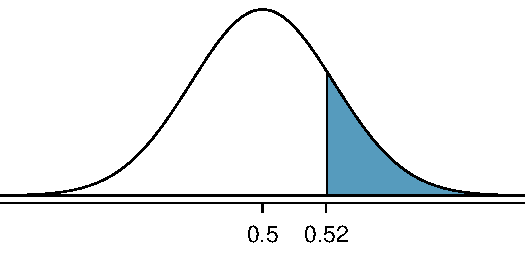
\includegraphics[width=0.5\textwidth]{06/figures/pValueForCampaignManagerClaimOfMoreThan50PercentSupport/pValueForCampaignManagerClaimOfMoreThan50PercentSupport}
\caption{Sampling distribution of the sample proportion if the null hypothesis is true for Example~\ref{TooheyInferenceExample}. The p-value for the test is shaded.}
\label{pValueForCampaignManagerClaimOfMoreThan50PercentSupport}
\end{figure}

\begin{termBox}{\tBoxTitle{Hypothesis test for a proportion}
Set up hypotheses and verify the conditions using the null value, $p_0$, to ensure $\hat{p}$ is nearly normal under $H_0$. If the conditions hold, construct the standard error, again using $p_0$, and show the p-value in a drawing. Lastly, compute the p-value and evaluate the hypotheses.}
\end{termBox}


\subsection{Choosing a sample size when estimating a proportion}

\index{margin of error|(}

Sample size computations are helpful in planning a study to control the size of the standard error of a point estimate for a single mean. The task is to find a sample size $n$ so that the sample mean is within some margin of error $m$ of the actual mean with a certain level of confidence. For example, the margin of error for a point estimate using 95\% confidence can be written as $1.96\times SE$. We set up a general equation to represent the problem:
\begin{align*}
ME = z^{\star}SE \leq m
\end{align*}
where $ME$ represented the actual margin of error and $z^{\star}$ is chosen to correspond to the confidence level. The standard error formula is specified to correspond to the particular setting. For instance, in the case of means, the standard error was given as $\sigma / \sqrt{n}$. In the case of a single proportion, we use $\sqrt{p(1-p) / n\ }$ for the standard error.

Planning a sample size before collecting data is equally important when estimating a proportion. For instance, if we are conducting a university survey to determine whether students support a \$200 per year increase in fees to pay for a new football stadium, how big of a sample is needed to be sure the margin of error is less than 0.04 using a 95\% confidence level?

\begin{example}{Find the smallest sample size $n$ so that the margin of error of the point estimate $\hat{p}$ will be no larger than $m=0.04$ when using a 95\% confidence interval.}
For a 95\% confidence level, the value $z^{\star}$ corresponds to 1.96, and we can write the margin of error expression as follows:
\begin{align*}
ME = z^{\star}SE = 1.96\times \sqrt{\frac{p(1-p)}{n}} \leq 0.04
\end{align*}
There are two unknowns in the equation: $p$ and $n$. If we have an estimate of $p$, perhaps from a similar survey, we could use that value. If we have no such estimate, we must use some other value for $p$. It turns out that the margin of error is largest when $p$ is 0.5, so we typically use this \emph{worst case estimate} if no other estimate is available:
\begin{align*}
	1.96\times \sqrt{\frac{0.5(1-0.5)}{n}} &\leq 0.04 \\
	1.96^2\times \frac{0.5(1-0.5)}{n} &\leq 0.04^2 \\
	1.96^2\times \frac{0.5(1-0.5)}{0.04^2} &\leq n \\
	600.25 &\leq n
\end{align*}
We would need at least 600.25 participants, which means we need 601 participants or more, to ensure the sample proportion is within 0.04 of the true proportion with 95\% confidence.
\end{example}

No estimate of the true proportion is required in sample size computations for a proportion, whereas an estimate of the standard deviation is always needed when computing a sample size for a margin of error for the sample mean. However, if we have an estimate of the proportion, we should use it in place of the worst case estimate of the proportion,~0.5.

\begin{exercise}
A manager is about to oversee the mass production of a new tire model in her factory, and she would like to estimate what proportion of these tires will be rejected through quality control. The quality control team has monitored the last three tire models produced by the factory, failing 1.7\% of tires in the first model, 6.2\% of the second model, and 1.3\% of the third model. The manager would like to examine enough tires to estimate the failure rate of the new tire model to within about 2\% with a 90\% confidence level.\footnote{(a) For the 1.7\% estimate of $p$, we estimate the appropriate sample size as follows:
\begin{align*}
1.65\times \sqrt{\frac{p(1-p)}{n}} \approx
1.65\times \sqrt{\frac{0.017(1-0.017)}{n}} &\leq 0.02 \qquad\to\qquad n \geq 113.7
\end{align*}
Using the estimate from the first model, we would suggest examining 114 tires (round up!). A similar computation can be accomplished using 0.062 and 0.013 for $p$: 396 and 88. \par
(b) We could examine which of the old models is most like the new model, then choose the corresponding sample size. Or if two of the previous estimates are based on small samples while the other is based on a larger sample, we should consider the value corresponding to the larger sample. (Answers will vary.)}
\begin{itemize}
\setlength{\itemsep}{0mm}
\item[(a)] There are three different failure rates to choose from. Perform the sample size computation for each separately, and identify three sample sizes to consider.
\item[(b)] The sample sizes in (b) vary widely. Which of the three would you suggest using? What would influence your choice?
\index{margin of error|)}
\end{itemize}
\end{exercise}

\index{data!Congress approval rating|(}

\begin{exercise}
A recent estimate of Congress' approval rating was 17\%.\footnote{\href{http://www.gallup.com/poll/155144/Congress-Approval-June.aspx}{www.gallup.com/poll/155144/Congress-Approval-June.aspx}} What sample size does this estimate suggest we should use for a margin of error of 0.04 with 95\% confidence?\footnote{We complete the same computations as before, except now we use $0.17$ instead of $0.5$ for $p$:
\begin{align*}
1.96\times \sqrt{\frac{p(1-p)}{n}} \approx
1.96\times \sqrt{\frac{0.17(1-0.17)}{n}} &\leq 0.04 \qquad\to\qquad n \geq 338.8
\end{align*}
A sample size of 339 or more would be reasonable.}

\index{data!Congress approval rating|)}

\end{exercise}


%__________________
\section{Difference of two proportions}
\label{differenceOfTwoProportions}

We would like to make conclusions about the difference in two population proportions: $p_1 - p_2$. We consider three examples. In the first, we compare the approval of the 2010 healthcare law under two different question phrasings. In the second application, a company weighs whether they should switch to a higher quality parts manufacturer. In the last example, we examine the cancer risk to dogs from the use of yard herbicides.

In our investigations, we first identify a reasonable point estimate of $p_1 - p_2$ based on the sample. You may have already guessed its form: $\hat{p}_1 - \hat{p}_2$\index{point estimate!difference of proportions}. Next, in each example we verify that the point estimate follows the normal model by checking certain conditions. Finally, we compute the estimate's standard error and apply our inferential framework.


\subsection{Sample distribution of the difference of two proportions}

We must check two conditions before applying the normal model to $\hat{p}_1 - \hat{p}_2$. First, the sampling distribution for each sample proportion must be nearly normal, and secondly, the samples must be independent. Under these two conditions, the sampling distribution of $\hat{p}_1 - \hat{p}_2$ may be well approximated using the normal model.

\begin{termBox}{\tBoxTitle{Conditions for the sampling distribution of $\hat{p}_1 - \hat{p}_2$ to be normal}
The difference $\hat{p}_1 - \hat{p}_2$ tends to follow a normal model when
\begin{itemize}
\setlength{\itemsep}{0mm}
\item each proportion separately follows a normal model, and
\item the samples are independent.
\end{itemize}
The standard error of the difference in sample proportions is
\index{standard error!difference in proportions}
\begin{eqnarray}
SE_{\hat{p}_1 - \hat{p}_2}
	= \sqrt{SE_{\hat{p}_1}^2 + SE_{\hat{p}_2}^2}
	= \sqrt{\frac{p_1(1-p_1)}{n_1} + \frac{p_2(1-p_2)}{n_2}}
\label{seForDiffOfProp}
\end{eqnarray}
where $p_1$ and $p_2$ represent the population proportions, and $n_1$ and $n_2$ represent the sample sizes.}
\end{termBox}

For the difference in two means, the standard error formula took the following form:
\begin{eqnarray*}
SE_{\bar{x}_{1} - \bar{x}_{2}} = \sqrt{SE_{\bar{x}_1}^2 + SE_{\bar{x}_2}^2}
\end{eqnarray*}
The standard error for the difference in two proportions takes a similar form. The reasons behind this similarity are rooted in the probability theory of Section~\ref{randomVariablesSection}, which is described for this context in Exercise~\vref{derivingSEForDiffOfTwoMeansExercise}.


\subsection{Intervals and tests for $p_1 -p_2$}

In the setting of confidence intervals, the sample proportions are used to verify the success-failure condition and also compute standard error, just as was the case with a single proportion.

\begin{example}{The way a question is phrased can influence a person's response. For example, Pew Research Center conducted a survey with the following question:\footnote{\href{http://www.people-press.org/2012/03/26/public-remains-split-on-health-care-bill-opposed-to-mandate/}{www.people-press.org/2012/03/26/public-remains-split-on-health-care-bill-opposed-to-mandate/}. Sample sizes for each polling group are approximate.}
\begin{quote}
As you may know, by 2014 nearly all Americans will be required to have health insurance. [People who do not buy insurance will pay a penalty] while [People who cannot afford it will receive financial help from the government]. Do you approve or disapprove of this policy?
\end{quote}
\index{data!health care|(}For each randomly sampled respondent, the statements in brackets were randomized: either they were kept in the order given above, or the two statements were reversed. Table~\ref{pewPollResultsForRandomizedStatementOrdering} shows the results of this experiment. Create and interpret a 90\% confidence interval of the difference in approval.}

\begin{table}[t]
\centering
\begin{tabular}{p{50mm}c p{13mm}p{14mm}p{16.5mm}c}
	&\ & Sample size ($n_i$) & Approve law (\%)	& Disapprove law (\%)	& Other \\
\hline
``people who cannot afford it will receive financial help from the government'' is given second \vspace{2.5mm}
	& & 771	& 47	& 49	& 3 \\
``people who do not buy it will pay a penalty'' is given second
	& & 732	& 34	& 63	& 3 \\
\hline
\end{tabular}
\caption{Results for a Pew Research Center poll where the ordering of two statements in a question regarding healthcare were randomized.\vspaceB{-2mm}}
\label{pewPollResultsForRandomizedStatementOrdering}
\end{table}

First the conditions must be verified. Because each group is a simple random sample from less than 10\% of the population, the observations are independent, both within the samples and between the samples. The success-failure condition also holds for each sample. Because all conditions are met, the normal model can be used for the point estimate of the difference in support, where $p_1$ corresponds to the original ordering and $p_2$ to the reversed ordering:
$$\hat{p}_{1} - \hat{p}_{2} = 0.47 - 0.34 = 0.13$$
The standard error may be computed from Equation~\eqref{seForDiffOfProp} using the sample proportions:
$$SE \approx \sqrt{\frac{0.47(1-0.47)}{771} + \frac{0.34(1-0.34)}{732}} = 0.025$$
For a 90\% confidence interval, we use $z^{\star} = 1.65$:
$$\text{point estimate} \ \pm\ z^{\star}SE \quad \to \quad 0.13 \ \pm\ 1.65 \times  0.025 \quad \to \quad (0.09, 0.17)$$
We are 90\% confident that the approval rating for the 2010 healthcare law changes between 9\% and 17\% due to the ordering of the two statements in the survey question. The Pew Research Center reported that this modestly large difference suggests that the opinions of much of the public are still fluid on the health insurance mandate.
\index{data!health care|)}
\end{example}

\begin{exercise}\label{carWheelGearManufacturer}
A remote control car company is considering a new manufacturer for wheel gears. The new manufacturer would be more expensive but their higher quality gears are more reliable, resulting in happier customers and fewer warranty claims. However, management must be convinced that the more expensive gears are worth the conversion before they approve the switch. If there is strong evidence of a more than 3\% improvement in the percent of gears that pass inspection, management says they will switch suppliers, otherwise they will maintain the current supplier. Set up appropriate hypotheses for the test.\footnote{$H_0$: The higher quality gears will pass inspection no more than 3\% more frequently than the standard quality gears. $p_{highQ} - p_{standard} = 0.03$. $H_A$: The higher quality gears will pass inspection more than 3\% more often than the standard quality gears. $p_{highQ} - p_{standard} > 0.03$.}
\end{exercise}

\begin{example}{The quality control engineer from Exercise~\ref{carWheelGearManufacturer} collects a sample of gears, examining 1000 gears from each company and finds that 899 gears pass inspection from the current supplier and 958 pass inspection from the prospective supplier. Using these data, evaluate the hypothesis setup of Exercise~\ref{carWheelGearManufacturer} using a significance level of 5\%.}
First, we check the conditions. The sample is not necessarily random, so to proceed we must assume the gears are all independent; for this sample we will suppose this assumption is reasonable, but the engineer would be more knowledgeable as to whether this assumption is appropriate. The success-failure condition also holds for each sample. Thus, the difference in sample proportions, $0.958-0.899=0.059$, can be said to come from a nearly normal distribution.

The standard error can be found using Equation~\eqref{seForDiffOfProp}:
$$SE = \sqrt{\frac{0.958(1-0.958)}{1000} + \frac{0.899(1-0.899)}{1000}} = 0.0114$$
In this hypothesis test, the sample proportions were used. We will discuss this choice more in Section~\ref{pooledHTForProportionsSection}.

Next, we compute the test statistic and use it to find the p-value, which is depicted in Figure~\ref{gearsTwoSampleHTPValueQC}.
$$Z = \frac{\text{point estimate} - \text{null value}}{SE} = \frac{0.059 - 0.03}{0.0114} = 2.54$$
Using the normal model for this test statistic, we identify the right tail area as 0.006. Since this is a one-sided test, this single tail area is also the p-value, and we reject the null hypothesis because 0.006 is less than 0.05. That is, we have statistically significant evidence that the higher quality gears actually do pass inspection more than 3\% as often as the currently used gears. Based on these results, management will approve the switch to the new supplier.
\end{example}

\begin{figure}
\centering
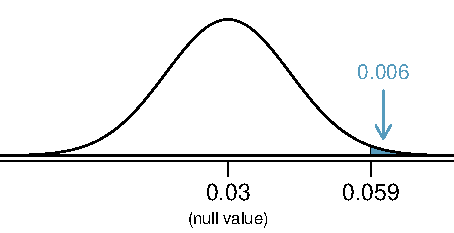
\includegraphics[width=0.5\textwidth]{06/figures/gearsTwoSampleHTPValueQC/gearsTwoSampleHTPValueQC}
\caption{Distribution of the test statistic if the null hypothesis was true. The p-value is represented by the shaded area.}
\label{gearsTwoSampleHTPValueQC}
\end{figure}

\textB{\newpage}

\subsection{Hypothesis testing when $H_0: p_1=p_2$}
\label{pooledHTForProportionsSection}

\index{data!cancer in dogs, herbicide|(}

Here we use a new example to examine a special estimate of standard error when $H_0: p_1 = p_2$. We investigate whether there is an increased risk of cancer in dogs that are exposed to the herbicide 2,4-dichlorophenoxyacetic acid (2,4-D). A study in 1994 examined 491 dogs that had developed cancer and 945 dogs as a control group.\footnote{Hayes HM, Tarone RE, Cantor KP, Jessen CR, McCurnin DM, and Richardson RC. 1991. Case-Control Study of Canine Malignant Lymphoma: Positive Association With Dog Owner's Use of 2, 4-Dichlorophenoxyacetic Acid Herbicides. Journal of the National Cancer Institute 83(17):1226-1231.} Of these two groups, researchers identified which dogs had been exposed to 2,4-D in their owner's yard. The results are shown in Table~\ref{24DAndCancerInDogs}.

\begin{table}[h]
\centering
\begin{tabular}{rrr}
  \hline
 & cancer & no cancer \\
  \hline
2,4-D & 191 & 304 \\
no 2,4-D & 300 & 641 \\
   \hline
\end{tabular}
\caption{Summary results for cancer in dogs and the use of 2,4-D by the dog's owner.}
\label{24DAndCancerInDogs}
\end{table}

\begin{exercise}
Is this study an experiment or an observational study?\footnote{The owners were not instructed to apply or not apply the herbicide, so this is an observational study. This question was especially tricky because one group was called the \emph{control group}, which is a term usually seen in experiments.}
\end{exercise}

\begin{exercise} \label{htFor24DAndCancerInDogs}
Set up hypotheses to test whether 2,4-D and the occurrence of cancer in dogs are related. Use a one-sided test and compare across the cancer and no cancer groups.\footnote{Using the proportions within the cancer and no cancer groups may seem odd. We intuitively may desire to compare the fraction of dogs with cancer in the 2,4-D and no 2,4-D groups, since the herbicide is an explanatory variable. However, the cancer rates in each group do not necessarily reflect the cancer rates in reality due to the way the data were collected. For this reason, computing cancer rates may greatly alarm dog owners. \\ $H_0$: the proportion of dogs with exposure to 2,4-D is the same in ``cancer'' and ``no cancer'' dogs, $p_c - p_n = 0$. \\ $H_A$: dogs with cancer are more likely to have been exposed to 2,4-D than dogs without cancer, $p_c - p_n > 0$.}
\end{exercise}

\textB{\newpage}

\begin{example}{Are the conditions met to use the normal model and make inference on the results?}\label{condFor24DAndCancerInDogsNormalInference}
(1) It is unclear whether this is a random sample. However, if we believe the dogs in both the cancer and no cancer groups are representative of each respective population and that the dogs in the study do not interact in any way, then we may find it reasonable to assume independence between observations. (2) The success-failure condition holds for each sample.

Under the assumption of independence, we can use the normal model and make statements regarding the canine population based on the data.
\end{example}

In your hypotheses for Exercise~\ref{htFor24DAndCancerInDogs}, the null is that the proportion of dogs with exposure to 2,4-D is the same in each group. The point estimate of the difference in sample proportions is $\hat{p}_c - \hat{p}_n = 0.067$. To identify the p-value for this test, we first check conditions (Example~\ref{condFor24DAndCancerInDogsNormalInference}) and compute the standard error of the difference:
$$SE = \sqrt{\frac{p_c(1-p_c)}{n_c} + \frac{p_n(1-p_n)}{n_n}}$$
In a hypothesis test, the distribution of the test statistic is always examined as though the null hypothesis is true, i.e. in this case, $p_c = p_n$. The standard error formula should reflect this equality in the null hypothesis. We will use $p$ to represent the common rate of dogs that are exposed to 2,4-D in the two groups:
$$SE = \sqrt{\frac{p(1-p)}{n_c} + \frac{p(1-p)}{n_n}}$$
We don't know the exposure rate, $p$, but we can obtain a good estimate of it by \emph{pooling} the results of both samples:
$$\hat{p} = \frac{\text{\# of ``successes''}}{\text{\# of cases}} = \frac{191 + 304}{191+300+304+641} = 0.345$$
This is called the \term{pooled estimate} of the sample proportion, and we use it to compute the standard error when the null hypothesis is that $p_1 = p_2$ (e.g. $p_c = p_n$ or $p_c - p_n = 0$). We also typically use it to verify the success-failure condition.

\begin{termBox}{\tBoxTitle{Pooled estimate of a proportion}
When the null hypothesis is $p_1 = p_2$, it is useful to find the pooled estimate of the shared proportion:
\begin{eqnarray*}
\hat{p} = \frac{\text{number of ``successes''}}{\text{number of cases}} = \frac{\hat{p}_1n_1 + \hat{p}_2n_2}{n_1 + n_2}
\end{eqnarray*}
Here $\hat{p}_1n_1$ represents the number of successes in sample 1 since
\begin{eqnarray*}
\hat{p}_1 = \frac{\text{number of successes in sample 1}}{n_1}
\end{eqnarray*}
Similarly, $\hat{p}_2n_2$ represents the number of successes in sample 2.}
\end{termBox}

\begin{tipBox}{\tipBoxTitle{Use the pooled proportion estimate when $\mathbf{H_0: p_1 = p_2}$}
When the null hypothesis suggests the proportions are equal, we use the pooled proportion estimate ($\hat{p}$) to verify the success-failure condition and also to estimate the standard error:
\begin{eqnarray}
SE = \sqrt{\frac{\hat{p}(1-\hat{p})}{n_c} + \frac{\hat{p}(1-\hat{p})}{n_n}} 
\label{seOfDiffInPropUsingPooledEstimate}
\end{eqnarray}}
\index{data!cancer in dogs, herbicide|)}
\end{tipBox}

\begin{exercise}\label{verifySEOfPooledEstimateOf24DWithCancerNoCancerDogs}
Using Equation~\eqref{seOfDiffInPropUsingPooledEstimate}, $\hat{p}=0.345$, $n_1 = 491$, and $n_2=945$, verify the estimate for the standard error is $SE = 0.026$. Next, complete the hypothesis test using a significance level of 0.05. Be certain to draw a picture, compute the p-value, and state your conclusion in both statistical language and plain language.\footnote{Compute the test statistic:
\begin{eqnarray*}
Z = \frac{\text{point estimate} - \text{null value}}{SE} = \frac{0.067 - 0}{0.026} = 2.58
\end{eqnarray*}
We leave the picture to you. Looking up $Z=2.58$ in the normal probability table: 0.9951. However this is the lower tail, and the upper tail represents the p-value: $1-0.9951 = 0.0049$. We reject the null hypothesis and conclude that dogs getting cancer and owners using 2,4-D are associated.}
\end{exercise}


%__________________
\section{Testing for goodness of fit using chi-square}
\label{oneWayChiSquare}

In this section, we develop a method for assessing a null model when the data are binned.
This technique is commonly used in two circumstances:
\begin{itemize}
\setlength{\itemsep}{0mm}
\item Given a sample of cases that can be classified into several groups, determine if the sample is representative of the general population.
\item Evaluate whether data resemble a particular distribution, such as a normal distribution or a geometric distribution.
\end{itemize}
Each of these scenarios can be addressed using the same statistical test: a chi-square test.

\index{data!racial make-up of jury|(}

In the first case, we consider data from a random sample of 275 jurors in a small county. Jurors identified their racial group, as shown in Table~\ref{juryRepresentationAndCityRepresentationForRace}, and we would like to determine if these jurors are racially representative of the population.  If the jury is representative of the population, then the proportions in the sample should roughly reflect the population of eligible jurors, i.e. registered voters.

\begin{table}[h]
\centering
\begin{tabular}{ll ccc c ll}
\hline
Race	 & \hspace{2mm} & White & Black & Hispanic & Other & \hspace{2mm} & Total \\
\hline
Representation in juries &	& 205 & 26 & 25 & 19 & & 275 \\
Registered voters	 & 		& 0.72 & 0.07 & 0.12 & 0.09 & & 1.00 \\
\hline
\end{tabular}
\caption{Representation by race in a city's juries and population.}
\label{juryRepresentationAndCityRepresentationForRace}
\end{table}

While the proportions in the juries do not precisely represent the population proportions, it is unclear whether these data provide convincing evidence that the sample is not representative. If the jurors really were randomly sampled from the registered voters, we might expect small differences due to chance. However, unusually large differences may provide convincing evidence that the juries were not representative.

A second application, assessing the fit of a distribution, is presented at the end of this section. Daily stock returns from the S\&P500 for the years 1990-2011 are used to assess whether stock activity each day is independent of the stock's behavior on previous days.

In these problems, we would like to examine all bins simultaneously, not simply compare one or two bins at a time, which will require us to develop a new test statistic.


\subsection{Creating a test statistic for one-way tables}

\begin{example}{Of the people in the city, 275 served on a jury. If the individuals are randomly selected to serve on a jury, about how many of the 275 people would we expect to be white? How many would we expect to be black?}
About 72\% of the population is white, so we would expect about 72\% of the jurors to be white: $0.72\times 275 = 198$.

Similarly, we would expect about 7\% of the jurors to be black, which would correspond to about $0.07\times 275 = 19.25$ black jurors.
\end{example}

\begin{exercise}
Twelve percent of the population is Hispanic and 9\% represent other races. How many of the 275 jurors would we expect to be Hispanic or from another race? Answers can be found in Table~\ref{expectedJuryRepresentationIfNoBias}.
\end{exercise}

\begin{table}[h]
\centering
\begin{tabular}{ll ccc c ll}
\hline
Race	 & \hspace{2mm} & White & Black & Hispanic & Other & \hspace{2mm} & Total \\
\hline
Observed data			&	& 205 & 26	& 25 & 19	&	& 275 \\
Expected counts	 &	& 198 & 19.25 & 33 & 24.75 & & 275 \\
\hline
\end{tabular}
\caption{Actual and expected make-up of the jurors.}
\label{expectedJuryRepresentationIfNoBias}
\end{table}

The sample proportion represented from each race among the 275 jurors was not a precise match for any ethnic group. While some sampling variation is expected, we would expect the sample proportions to be fairly similar to the population proportions if there is no bias on juries. We need to test whether the differences are strong enough to provide convincing evidence that the jurors are not a random sample. These ideas can be organized into hypotheses:
\begin{itemize}
\setlength{\itemsep}{0mm}
\item[$H_0$:] The jurors are a random sample, i.e. there is no racial bias in who serves on a jury, and the observed counts reflect natural sampling fluctuation.
\item[$H_A$:] The jurors are not randomly sampled, i.e. there is racial bias in juror selection.
\end{itemize}
To evaluate these hypotheses, we quantify how different the observed counts are from the expected counts. Strong evidence for the alternative hypothesis would come in the form of unusually large deviations in the groups from what would be expected based on sampling variation alone.


\subsection{The chi-square test statistic}
\label{chiSquareTestStatistic}

In previous hypothesis tests, we constructed a test statistic of the following form:
$$ \frac{\text{point estimate} - \text{null value}}{\text{SE of point estimate}} $$
This construction was based on (1) identifying the difference between a point estimate and an expected value if the null hypothesis was true, and (2) standardizing that difference using the standard error of the point estimate. These two ideas will help in the construction of an appropriate test statistic for count data.

Our strategy will be to first compute the difference between the observed counts and the counts we would expect if the null hypothesis was true, then we will standardize the difference:
\begin{align*}
Z_{1} = \frac{\text{observed white count} - \text{null white count}}
				{\text{SE of observed white count}}
\end{align*}
The standard error for the point estimate of the count in binned data is the square root of the count under the null.\footnote{Using some of the rules learned in earlier chapters, we might think that the standard error would be $np(1-p)$, where $n$ is the sample size and $p$ is the proportion in the population. This would be correct if we were looking only at one count. However, we are computing many standardized differences and adding them together. It can be shown -- though not here -- that the square root of the count is a better way to standardize the count differences.} Therefore:
\begin{align*}
Z_1 = \frac{205 - 198}{\sqrt{198}} = 0.50
\end{align*}
The fraction is very similar to previous test statistics: first compute a difference, then standardize it. These computations should also be completed for the black, Hispanic, and other groups:
\begin{align*}
&Black && Hispanic	&&Other \\
& Z_2 = \frac{26-19.25}{\sqrt{19.25}}=1.54\ \ \ \ 
	&& Z_3 = \frac{25-33}{\sqrt{33}}=-1.39\ \ \ \ 
	&& Z_4 = \frac{19-24.75}{\sqrt{24.75}}=-1.16 \\
\end{align*}
We would like to use a single test statistic to determine if these four standardized differences are irregularly far from zero. That is, $Z_1$, $Z_2$, $Z_3$, and $Z_4$ must be combined somehow to help determine if they -- as a group -- tend to be unusually far from zero. A first thought might be to take the absolute value of these four standardized differences and add them~up:
\begin{align*}
|Z_1| + |Z_2| + |Z_3| + |Z_4| = 4.58
\end{align*}
Indeed, this does give one number summarizing how far the actual counts are from what was expected. However, it is more common to add the squared values:
\begin{align*}
Z_1^2 + Z_2^2 + Z_3^2 + Z_4^2 = 5.89
\end{align*}
Squaring each standardized difference before adding them together does two things:
\begin{itemize}
\setlength{\itemsep}{0mm}
\item Any standardized difference that is squared will now be positive.
\item Differences that already look unusual -- e.g. a standardized difference of 2.5 -- will become much larger after being squared.
\end{itemize}
The test statistic $X^2$\marginpar[\raggedright\vspace{9mm}

$X^2$\vspace{0.5mm}\\\footnotesize chi-square\\test statistic]{\raggedright\vspace{9mm}

$X^2$\vspace{0.5mm}\\\footnotesize chi-square\\test statistic}, which is the sum of the $Z^2$ values, is generally used for these reasons. We can also write an equation for $X^2$ using the observed counts and null counts:
\index{data!racial make-up of jury|)}
{\begin{align*}
X^2 &=
	\frac
	{\text{\footnotesize$(\text{observed count}_1 - \text{null count}_1)^2$}}
	{\text{\footnotesize$\text{null count}_1$}}
	+ \dots + \frac
	{\text{\footnotesize$(\text{observed count}_4 - \text{null count}_4)^2$}}
	{\text{\footnotesize$\text{null count}_4$}}
\end{align*}
}The final number $X^2$ summarizes how strongly the observed counts tend to deviate from the null counts. In Section~\ref{pValueForAChiSquareTest}, we will see that if the null hypothesis is true, then $X^2$ follows a new distribution called a \emph{chi-square distribution}. Using this distribution, we will be able to obtain a p-value to evaluate the hypotheses.


\subsection{The chi-square distribution and finding areas}

The \term{chi-square distribution} is sometimes used to characterize data sets and statistics that are always positive and typically right skewed. Recall the normal distribution had two parameters -- mean and standard deviation -- that could be used to describe its exact characteristics. The chi-square distribution has just one parameter called \termsub{degrees of freedom (df)}{degrees of freedom (df)!chi-square}, which influences the shape, center, and spread of the distribution.

\begin{exercise}\label{exerChiSquareDistributionDescriptionWithMoreDOF}
Figure~\ref{chiSquareDistributionWithInceasingDF} shows three chi-square distributions. (a) How does the center of the distribution change when the degrees of freedom is larger? (b) What about the variability (spread)? (c) How does the shape change?\footnote{(a)~The center becomes larger. If we look carefully, we can see that the center of each distribution is equal to the distribution's degrees of freedom. (b)~The variability increases as the degrees of freedom increases. (c)~The distribution is very strongly skewed for $df=2$, and then the distributions become more symmetric for the larger degrees of freedom $df=4$ and $df=9$. We would see this trend continue if we examined distributions with even more larger degrees of freedom.}
\end{exercise}

\begin{figure}[h]
\centering
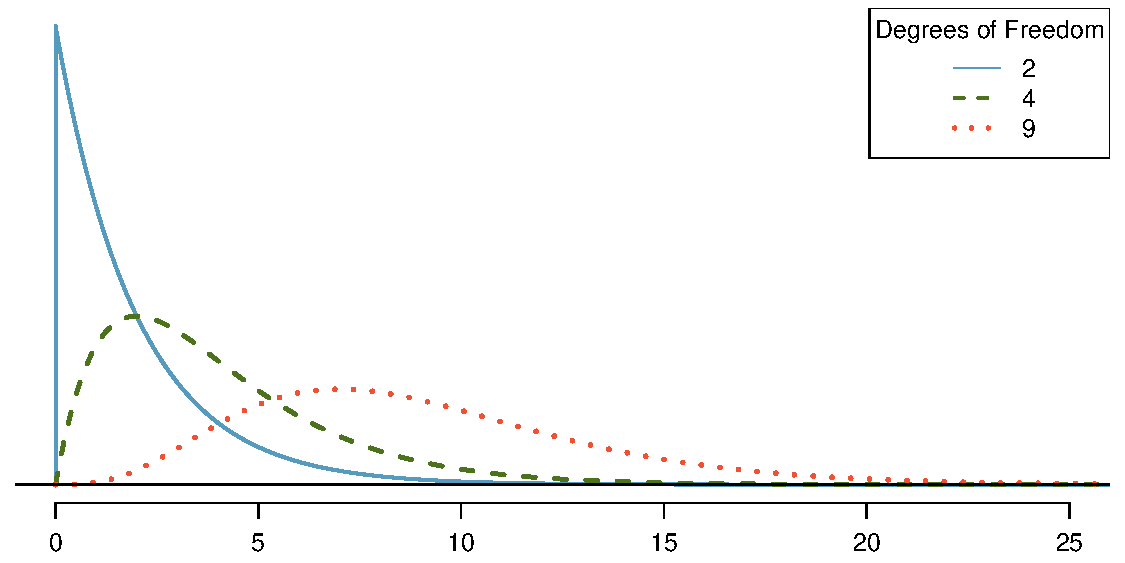
\includegraphics[width=0.9\textwidth]{06/figures/chiSquareDistributionWithInceasingDF/chiSquareDistributionWithInceasingDF}
\caption{Three chi-square distributions with varying degrees of freedom.}
\label{chiSquareDistributionWithInceasingDF}
\end{figure}

Figure~\ref{chiSquareDistributionWithInceasingDF} and Exercise~\ref{exerChiSquareDistributionDescriptionWithMoreDOF} demonstrate three general properties of chi-square distributions as the degrees of freedom increases: the distribution becomes more symmetric, the center moves to the right, and the variability inflates.

Our principal interest in the chi-square distribution is the calculation of p-values, which (as we have seen before) is related to finding the relevant area in the tail of a distribution. To do so, a new table is needed: the \term{chi-square table}, partially shown in Table~\ref{chiSquareProbabilityTableShort}. A more complete table is presented in Appendix~\vref{chiSquareProbabilityTable}. This table is very similar to the $t$ table from Section~\ref{oneSampleMeansWithTDistribution}: we identify a range for the area, and we examine a particular row for distributions with different degrees of freedom. One important difference from the $t$ table is that the chi-square table only provides upper tail values.

\begin{table}[h]
\centering
\begin{tabular}{r | rrrr | rrrr |}
  \hline
Upper tail & 0.3 & 0.2 & 0.1 & 0.05 & 0.02 & 0.01 & 0.005 & 0.001 \\ 
  \hline
%df \hfill 1 & \footnotesize 1.07 & \footnotesize 1.64 & \footnotesize 2.71 & \footnotesize 3.84 & \footnotesize 5.41 & \footnotesize 6.63 & \footnotesize 7.88 & \footnotesize 10.83 \\ 
df \hfill 2 & \footnotesize 2.41 & \footnotesize \highlightO{3.22} & \footnotesize \highlightO{4.61} & \footnotesize 5.99 & \footnotesize 7.82 & \footnotesize 9.21 & \footnotesize 10.60 & \footnotesize 13.82 \\ 
  \em3 & \em\footnotesize 3.66 & \em\footnotesize 4.64 & \em\footnotesize \highlightT{6.25} & \em\footnotesize 7.81 & \em\footnotesize 9.84 & \em\footnotesize 11.34 & \em\footnotesize 12.84 & \em\footnotesize 16.27 \\ 
  4 & \footnotesize 4.88 & \footnotesize 5.99 & \footnotesize 7.78 & \footnotesize 9.49 & \footnotesize 11.67 & \footnotesize 13.28 & \footnotesize 14.86 & \footnotesize 18.47 \\ 
  5 & \footnotesize 6.06 & \footnotesize 7.29 & \footnotesize 9.24 & \footnotesize 11.07 & \footnotesize 13.39 & \footnotesize 15.09 & \footnotesize 16.75 & \footnotesize 20.52 \\ 
  \hline
  6 & \footnotesize 7.23 & \footnotesize 8.56 & \footnotesize 10.64 & \footnotesize 12.59 & \footnotesize 15.03 & \footnotesize 16.81 & \footnotesize 18.55 & \footnotesize 22.46 \\ 
  7 & \footnotesize 8.38 & \footnotesize 9.80 & \footnotesize 12.02 & \footnotesize 14.07 & \footnotesize 16.62 & \footnotesize 18.48 & \footnotesize 20.28 & \footnotesize 24.32 \\ 
  \hline
\end{tabular}
\caption{A section of the chi-square table. A complete table is in Appendix~\vref{chiSquareProbabilityTable}.}
\label{chiSquareProbabilityTableShort}
\end{table}

\begin{example}{Figure~\ref{chiSquareAreaAbove6Point25WithDF3} shows a chi-square distribution with 3 degrees of freedom and an upper shaded tail starting at 6.25. Use Table~\ref{chiSquareProbabilityTableShort} to estimate the shaded area.}
This distribution has three degrees of freedom, so only the row with 3 degrees of freedom (df) is relevant. This row has been italicized in the table. Next, we see that the value -- 6.25 -- falls in the column with upper tail area 0.1. That is, the shaded upper tail of Figure~\ref{chiSquareAreaAbove6Point25WithDF3} has area 0.1.
\end{example}

\begin{figure}
\centering
\subfigure[]{
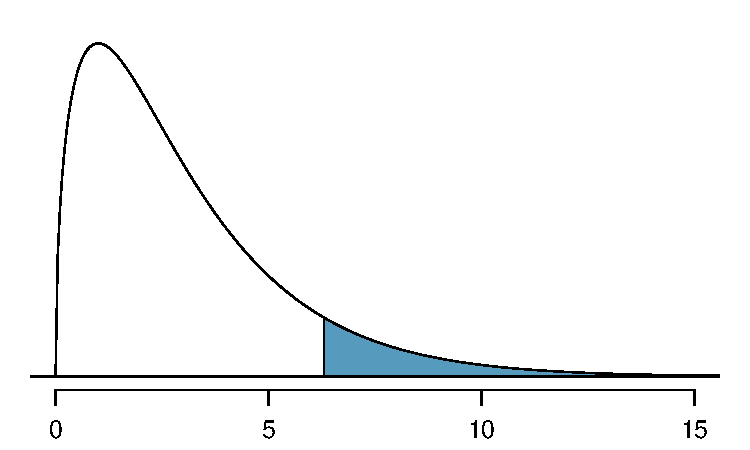
\includegraphics[width=0.475\textwidth]{06/figures/arrayOfFigureAreasForChiSquareDistribution/chiSquareAreaAbove6Point25WithDF3/chiSquareAreaAbove6Point25WithDF3}
\label{chiSquareAreaAbove6Point25WithDF3}
}
\subfigure[]{
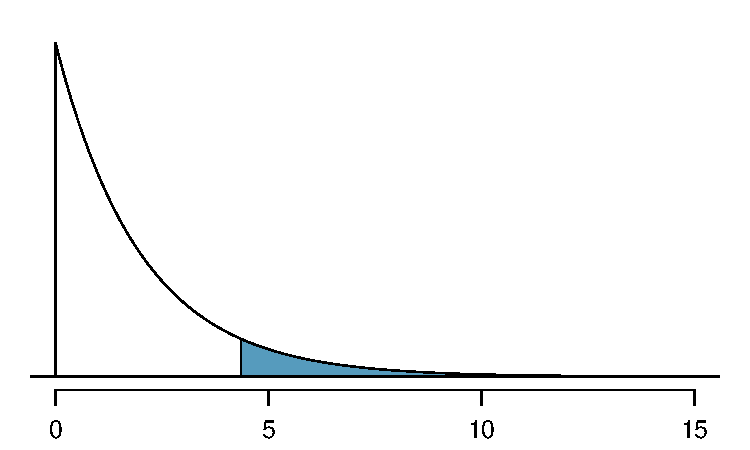
\includegraphics[width=0.475\textwidth]{06/figures/arrayOfFigureAreasForChiSquareDistribution/chiSquareAreaAbove4Point3WithDF2/chiSquareAreaAbove4Point3WithDF2}
\label{chiSquareAreaAbove4Point3WithDF2}
}
\subfigure[]{
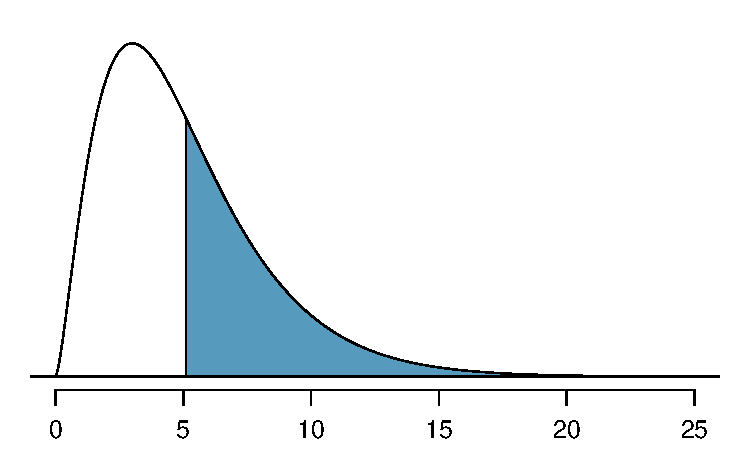
\includegraphics[width=0.475\textwidth]{06/figures/arrayOfFigureAreasForChiSquareDistribution/chiSquareAreaAbove5Point1WithDF5/chiSquareAreaAbove5Point1WithDF5}
\label{chiSquareAreaAbove5Point1WithDF5}
}
\subfigure[]{
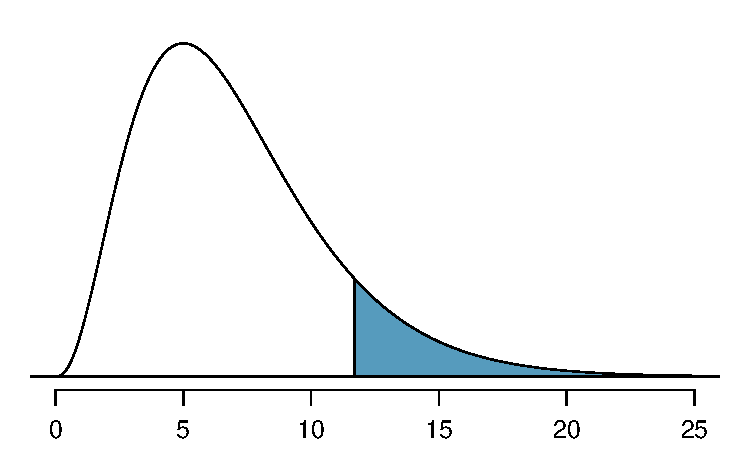
\includegraphics[width=0.475\textwidth]{06/figures/arrayOfFigureAreasForChiSquareDistribution/chiSquareAreaAbove11Point7WithDF7/chiSquareAreaAbove11Point7WithDF7}
\label{chiSquareAreaAbove11Point7WithDF7}
}
\subfigure[]{
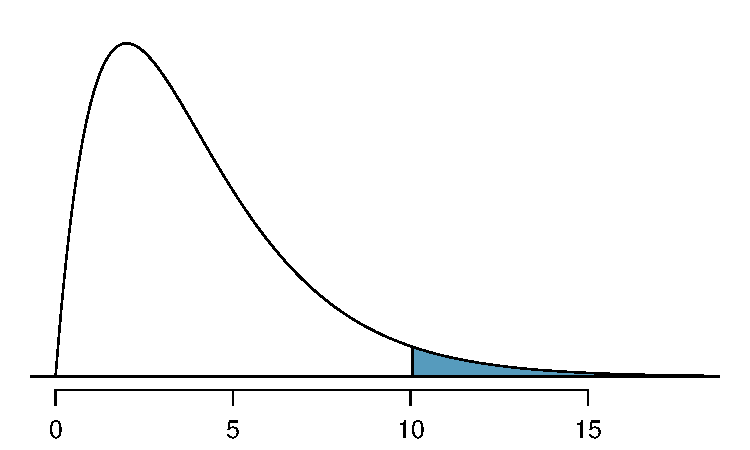
\includegraphics[width=0.475\textwidth]{06/figures/arrayOfFigureAreasForChiSquareDistribution/chiSquareAreaAbove10WithDF4/chiSquareAreaAbove10WithDF4}
\label{chiSquareAreaAbove10WithDF4}
}
\subfigure[]{
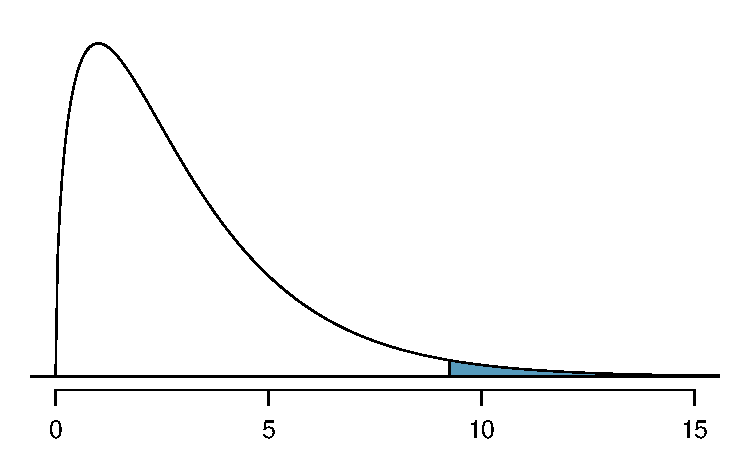
\includegraphics[width=0.475\textwidth]{06/figures/arrayOfFigureAreasForChiSquareDistribution/chiSquareAreaAbove9Point21WithDF3/chiSquareAreaAbove9Point21WithDF3}
\label{chiSquareAreaAbove9Point21WithDF3}
}
\caption{\textbf{\subref{chiSquareAreaAbove6Point25WithDF3}} Chi-square distribution with 3 degrees of freedom, area above 6.25 shaded. \textbf{\subref{chiSquareAreaAbove4Point3WithDF2}} 2 degrees of freedom, area above 4.3 shaded. \textbf{\subref{chiSquareAreaAbove5Point1WithDF5}} 5 degrees of freedom, area above 5.1 shaded. \textbf{\subref{chiSquareAreaAbove11Point7WithDF7}} 7 degrees of freedom, area above 11.7 shaded. \textbf{\subref{chiSquareAreaAbove10WithDF4}} 4 degrees of freedom, area above 10 shaded. \textbf{\subref{chiSquareAreaAbove9Point21WithDF3}} 3 degrees of freedom, area above 9.21 shaded.}
\label{arrayOfFigureAreasForChiSquareDistribution}
\end{figure}

\begin{example}{We rarely observe the \emph{exact} value in the table. For instance, Figure~\ref{chiSquareAreaAbove4Point3WithDF2} shows the upper tail of a chi-square distribution with 2 degrees of freedom. The bound for this upper tail is at 4.3, which does not fall in Table~\ref{chiSquareProbabilityTableShort}. Find the approximate tail area.}
The cutoff 4.3 falls between the second and third columns in the 2 degrees of freedom row. Because these columns correspond to tail areas of 0.2 and 0.1, we can be certain that the area shaded in Figure~\ref{chiSquareAreaAbove4Point3WithDF2} is between 0.1 and 0.2.
\end{example}

\begin{example}{Figure~\ref{chiSquareAreaAbove5Point1WithDF5} shows an upper tail for a chi-square distribution with 5 degrees of freedom and a cutoff of 5.1. Find the tail area.}
Looking in the row with 5 df, 5.1 falls below the smallest cutoff for this row (6.06). That means we can only say that the area is \emph{greater than 0.3}.
\end{example}

\begin{exercise}
Figure~\ref{chiSquareAreaAbove11Point7WithDF7} shows a cutoff of 11.7 on a chi-square distribution with 7 degrees of freedom. Find the area of the upper tail.\footnote{The value 11.7 falls between 9.80 and 12.02 in the 7 df row. Thus, the area is between 0.1 and 0.2.}
\end{exercise}

\begin{exercise}
Figure~\ref{chiSquareAreaAbove10WithDF4} shows a cutoff of 10 on a chi-square distribution with 4 degrees of freedom. Find the area of the upper tail.\footnote{The area is between 0.02 and 0.05.}
\end{exercise}

\begin{exercise}
Figure~\ref{chiSquareAreaAbove9Point21WithDF3} shows a cutoff of 9.21 with a chi-square distribution with 3 df. Find the area of the upper tail.\footnote{Between 0.02 and 0.05.}
\end{exercise}


\subsection{Finding a p-value for a chi-square distribution}
\label{pValueForAChiSquareTest}

\index{data!racial make-up of jury|(}
In Section~\ref{chiSquareTestStatistic}, we identified a new test statistic ($X^2$) within the context of assessing whether there was evidence of racial bias in how jurors were sampled. The null hypothesis represented the claim that jurors were randomly sampled and there was no racial bias. The alternative hypothesis was that there was racial bias in how the jurors were sampled.

We determined that a large $X^2$ value would suggest strong evidence favoring the alternative hypothesis: that there was racial bias. However, we could not quantify what the chance was of observing such a large test statistic ($X^2=5.89$) if the null hypothesis actually was true. This is where the chi-square distribution becomes useful. If the null hypothesis was true and there was no racial bias, then $X^2$ would follow a chi-square distribution, with three degrees of freedom in this case. Under certain conditions, the statistic $X^2$ follows a chi-square distribution with $k-1$ degrees of freedom, where $k$ is the number of bins.

\begin{example}{How many categories were there in the juror example? How many degrees of freedom should be associated with the chi-square distribution used for $X^2$?}
In the jurors example, there were $k=4$ categories: white, black, Hispanic, and other. According to the rule above, the test statistic $X^2$ should then follow a chi-square distribution with $k-1 = 3$ degrees of freedom if $H_0$ is true.
\end{example}

Just like we checked sample size conditions to use the normal model in earlier sections, we must also check a sample size condition to safely apply the chi-square distribution for $X^2$. Each expected count must be at least 5. In the juror example, the expected counts were 198, 19.25, 33, and 24.75, all easily above~5, so we can apply the chi-square model to the test statistic, $X^2=5.89$.

\begin{example}{If the null hypothesis is true, the test statistic $X^2=5.89$ would be closely associated with a chi-square distribution with three degrees of freedom. Using this distribution and test statistic, identify the p-value.}
The chi-square distribution and p-value are shown in Figure~\ref{jurorHTPValueShown}. Because larger chi-square values correspond to stronger evidence against the null hypothesis, we shade the upper tail to represent the p-value. Using the chi-square table in Appendix~\ref{chiSquareProbabilityTable} or the short table on page~\pageref{chiSquareProbabilityTableShort}, we can determine that the area is between 0.1 and 0.2. That is, the p-value is larger than 0.1 but smaller than 0.2. Generally we do not reject the null hypothesis with such a large p-value. In other words, the data do not provide convincing evidence of racial bias in the juror selection.
\index{data!racial make-up of jury|)}
\end{example}

\begin{figure}[h]
\centering
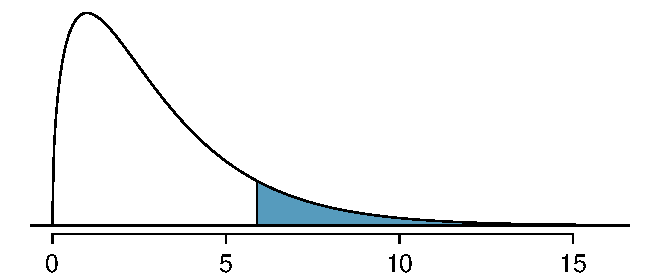
\includegraphics[width=0.61\textwidth]{06/figures/jurorHTPValueShown/jurorHTPValueShown}
\caption{The p-value for the juror hypothesis test is shaded in the chi-square distribution with $df=3$.}
\label{jurorHTPValueShown}
\end{figure}

\begin{termBox}{\tBoxTitle{Chi-square test for one-way table}
Suppose we are to evaluate whether there is convincing evidence that a set of observed counts $O_1$, $O_2$, ..., $O_k$ in $k$ categories are unusually different from what might be expected under a null hypothesis. Call the \emph{expected counts} that are based on the null hypothesis $E_1$, $E_2$, ..., $E_k$. If each expected count is at least 5 and the null hypothesis is true, then the test statistic below follows a chi-square distribution with $k-1$ degrees of freedom:
\begin{align*}
X^2 = \frac{(O_1 - E_1)^2}{E_1} + \frac{(O_2 - E_2)^2}{E_2} + \cdots + \frac{(O_k - E_k)^2}{E_k}
\end{align*}
The p-value for this test statistic is found by looking at the upper tail of this chi-square distribution. We consider the upper tail because larger values of $X^2$ would provide greater evidence against the null hypothesis.}
\end{termBox}

\begin{tipBox}{\tipBoxTitle{Conditions for the chi-square test}
There are three conditions that must be checked before performing a chi-square test:\vspace{-1mm}
\begin{description}
\setlength{\itemsep}{0mm}
\item[Independence.] Each case that contributes a count to the table must be independent of all the other cases in the table.
\item[Sample size / distribution.] Each particular scenario (i.e. cell count) must have at least 5~expected cases.
\item[Degrees of freedom] We only apply the chi-square technique when the table is associated with a chi-square distribution with 2 or more degrees of freedom. \vspace{-1mm}
\end{description}
Failing to check conditions may affect the test's error rates.}
\end{tipBox}

When examining a table with just two bins, pick a single bin and use the one-proportion methods introduced in Section~\ref{singleProportion}.


\subsection{Evaluating goodness of fit for a distribution}

\index{data!S\&P500 stock data|(}

We can apply our new chi-square testing framework to the second problem in this section: evaluating whether a certain statistical model fits a data set. Daily stock returns from the S\&P500 for 1990-2011 can be used to assess whether stock activity each day is independent of the stock's behavior on previous days. This sounds like a very complex question, and it is, but a chi-square test can be used to study the problem. We will label each day as \resp{Up} or \resp{Down} (\resp{D}) depending on whether the market was up or down that day. For example, consider the following changes in price, their new labels of up and down, and then the number of days that must be observed before each \resp{Up} day:
\begin{center}\footnotesize
\begin{tabular}{lc ccc ccc ccc cc}
Change in price		&\hspace{-1mm}	& \footnotesize2.52 &
	\footnotesize-1.46 & \footnotesize 0.51 &
	\footnotesize-4.07 & \footnotesize3.36 &
	\footnotesize1.10 &
	\footnotesize-5.46 & \footnotesize-1.03 & \footnotesize-2.99 & \footnotesize1.71 \\
Outcome	 & \hspace{-1mm} &
	Up &
	D & Up &
	D & Up &
	Up &
	D & D & D & Up \\
\footnotesize Days to Up & \hspace{-1mm} & 1 & - & 2 & - & 2 & 1 & - & - & - & 4 \\
\end{tabular}
\end{center}
If the days really are independent, then the number of days until a positive trading day should follow a geometric distribution. The geometric distribution describes the probability of waiting for the $k^{th}$ trial to observe the first success. Here each up day (Up) represents a success, and down (D) days represent failures. In the data above, it took only one day until the market was up, so the first wait time was 1 day. It took two more days before we observed our next \resp{Up} trading day, and two more for the third \resp{Up} day. We would like to determine if these counts (1, 2, 2, 1, 4, and so on) follow the geometric distribution. Table~\ref{sAndP500For1990To2011TimeToPosTrade} shows the number of waiting days for a positive trading day during 1990-2011 for the S\&P500.

\begin{table}[h]
\centering
\begin{tabular}{ll ccc ccc c ll}
\hline
Days	 & \hspace{2mm} & 1 & 2 & 3 & 4 & 5 & 6 & 7+ & \hspace{2mm} & Total \\
Observed &		& 1532 & 760 & 338 & 194 & 74 & 33 & 17 & & 2948 \\
\hline
\end{tabular}
\caption{Observed distribution of the waiting time until a positive trading day for the S\&P500, 1990-2011.}
\label{sAndP500For1990To2011TimeToPosTrade}
\end{table}

We consider how many days one must wait until observing an \resp{Up} day on the S\&P500 stock exchange. If the stock activity was independent from one day to the next and the probability of a positive trading day was constant, then we would expect this waiting time to follow a \emph{geometric distribution}. We can organize this into a hypothesis framework:
\begin{itemize}
\item[$H_0$:] The stock market being up or down on a given day is independent from all other days. We will consider the number of days that pass until an \resp{Up} day is observed. Under this hypothesis, the number of days until an \resp{Up} day should follow a geometric distribution.
\item[$H_A$:] The stock market being up or down on a given day is not independent from all other days. Since we know the number of days until an \resp{Up} day would follow a geometric distribution under the null, we look for deviations from the geometric distribution, which would support the alternative hypothesis.
\end{itemize}
There are important implications in our result for stock traders: if information from past trading days is useful in telling what will happen today, that information may provide an advantage over other traders.

We consider data for the S\&P500 from 1990 to 2011 and summarize the waiting times in Table~\ref{sAndP500For1990To2011TimeToPosTrade2} and Figure~\ref{geomFitEvaluationForSP500For1990To2011}. The S\&P500 was positive on 53.2\% of those days.

\begin{table}
\centering
\begin{tabular}{ll ccc ccc c ll}
\hline
Days	 & \hspace{1mm} & 1 & 2 & 3 & 4 & 5 & 6 & 7+ & \hspace{1mm} & Total \\
\hline
Observed &		& 1532 & 760 & 338 & 194 & 74 & 33 & 17 & & 2948 \\
Geometric Model &		& 1569 & 734 & 343 & 161 & 75 & 35 & 31 & & 2948 \\
\hline
\end{tabular}
\caption{Distribution of the waiting time until a positive trading day. The expected counts based on the geometric model are shown in the last row. To find each expected count, we identify the probability of waiting $D$ days based on the geometric model ($P(D) = (1-0.532)^{D-1}(0.532)$) and multiply by the total number of streaks, 2948. For example, waiting for three days occurs under the geometric model about $0.468^2\times 0.532 = 11.65\%$ of the time, which corresponds to $0.1165\times 2948 = 343$ streaks.}
\label{sAndP500For1990To2011TimeToPosTrade2}
\end{table}

\begin{figure}
\centering
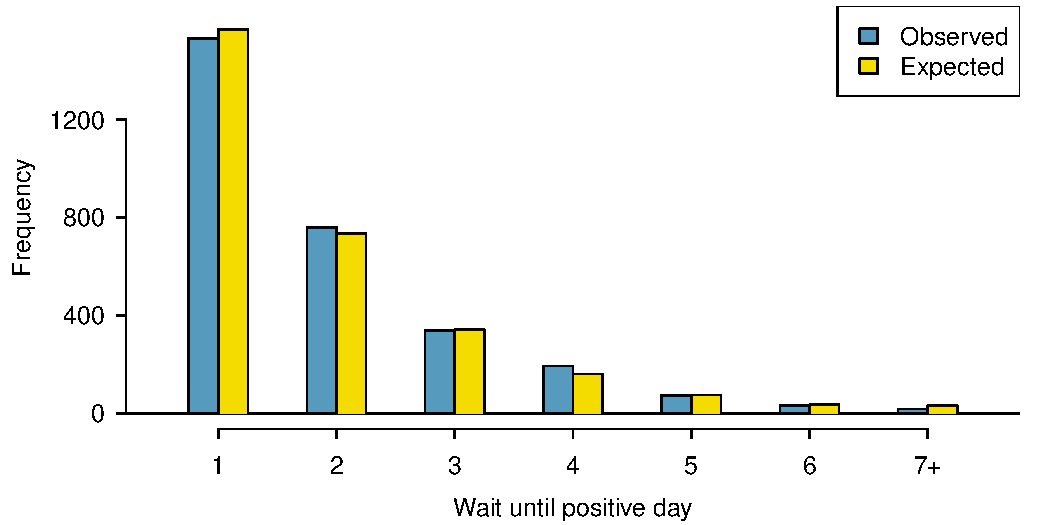
\includegraphics[width=0.98\textwidth]{06/figures/geomFitEvaluationForSP500For1990To2011/geomFitEvaluationForSP500For1990To2011}
\caption{Side-by-side bar plot of the observed and expected counts for each waiting time.}
\label{geomFitEvaluationForSP500For1990To2011}
\end{figure}

Because applying the chi-square framework requires expected counts to be at least~5, we have \emph{binned} together all the cases where the waiting time was at least 7 days to ensure each expected count is well above this minimum. The actual data, shown in the \emph{Observed} row in Table~\ref{sAndP500For1990To2011TimeToPosTrade2}, can be compared to the expected counts from the \emph{Geometric Model} row. The method for computing expected counts is discussed in Table~\ref{sAndP500For1990To2011TimeToPosTrade2}. In general, the expected counts are determined by (1) identifying the null proportion associated with each bin, then (2) multiplying each null proportion by the total count to obtain the expected counts. That is, this strategy identifies what proportion of the total count we would expect to be in each bin.

\begin{example}{Do you notice any unusually large deviations in the graph? Can you tell if these deviations are due to chance just by looking?}
It is not obvious whether differences in the observed counts and the expected counts from the geometric distribution are significantly different. That is, it is not clear whether these deviations might be due to chance or whether they are so strong that the data provide convincing evidence against the null hypothesis. However, we can perform a chi-square test using the counts in Table~\ref{sAndP500For1990To2011TimeToPosTrade2}.
\end{example}

\begin{exercise}
Table~\ref{sAndP500For1990To2011TimeToPosTrade2} provides a set of count data for waiting times ($O_1=1532$, $O_2=760$, ...) and expected counts under the geometric distribution ($E_1=1569$, $E_2=734$, ...). Compute the chi-square test statistic, $X^2$.\footnote{$X^2=\frac{(1532-1569)^2}{1569} + \frac{(760-734)^2}{734} + \cdots + \frac{(17-31)^2}{31} = 15.08$}
\end{exercise}

\begin{exercise}
Because the expected counts are all at least~5, we can safely apply the chi-square distribution to $X^2$. However, how many degrees of freedom should we~use?\footnote{There are $k=7$ groups, so we use $df=k-1=6$.}
\end{exercise}

\begin{example}{If the observed counts follow the geometric model, then the chi-square test statistic $X^2=15.08$ would closely follow a chi-square distribution with $df=6$. Using this information, compute a p-value.} \label{RejectGeomModelForSP500StockDataFor1990To2011}
Figure~\ref{geomFitPValueForSP500For1990To2011} shows the chi-square distribution, cutoff, and the shaded p-value. If we look up the statistic $X^2=15.08$ in Appendix~\ref{chiSquareProbabilityTable}, we find that the p-value is between 0.01 and 0.02. In other words, we have sufficient evidence to reject the notion that the wait times follow a geometric distribution, i.e. trading days are not independent and past days may help predict what the stock market will do today.
\end{example}

\begin{figure}
\centering
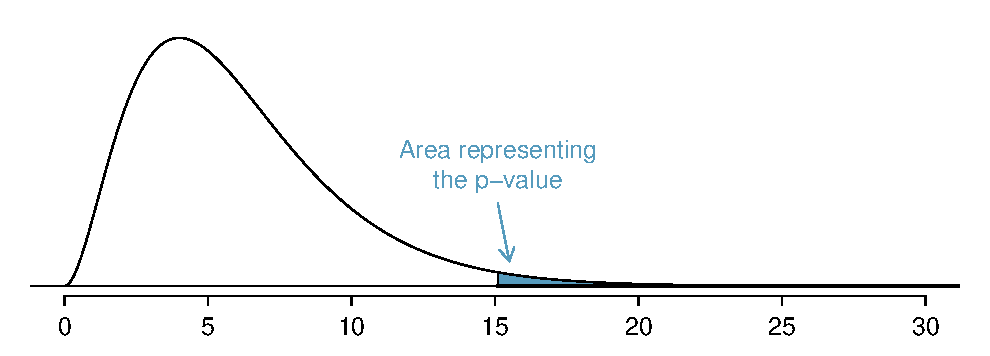
\includegraphics[width=0.97\textwidth]{06/figures/geomFitPValueForSP500For1990To2011/geomFitPValueForSP500For1990To2011}
\caption{Chi-square distribution with 6 degrees of freedom. The p-value for the stock analysis is shaded.}
\label{geomFitPValueForSP500For1990To2011}
\end{figure}

\begin{example}{In Example~\ref{RejectGeomModelForSP500StockDataFor1990To2011}, we rejected the null hypothesis that the trading days are independent. Why is this so important?}
Because the data provided strong evidence that the geometric distribution is not appropriate, we reject the claim that trading days are independent. While it is not obvious how to exploit this information, it suggests there are some hidden patterns in the data that could be interesting and possibly useful to a stock trader.
\index{data!S\&P500 stock data|)}
\end{example}




